\section{Numerical Approaches}

\begin{figure*}
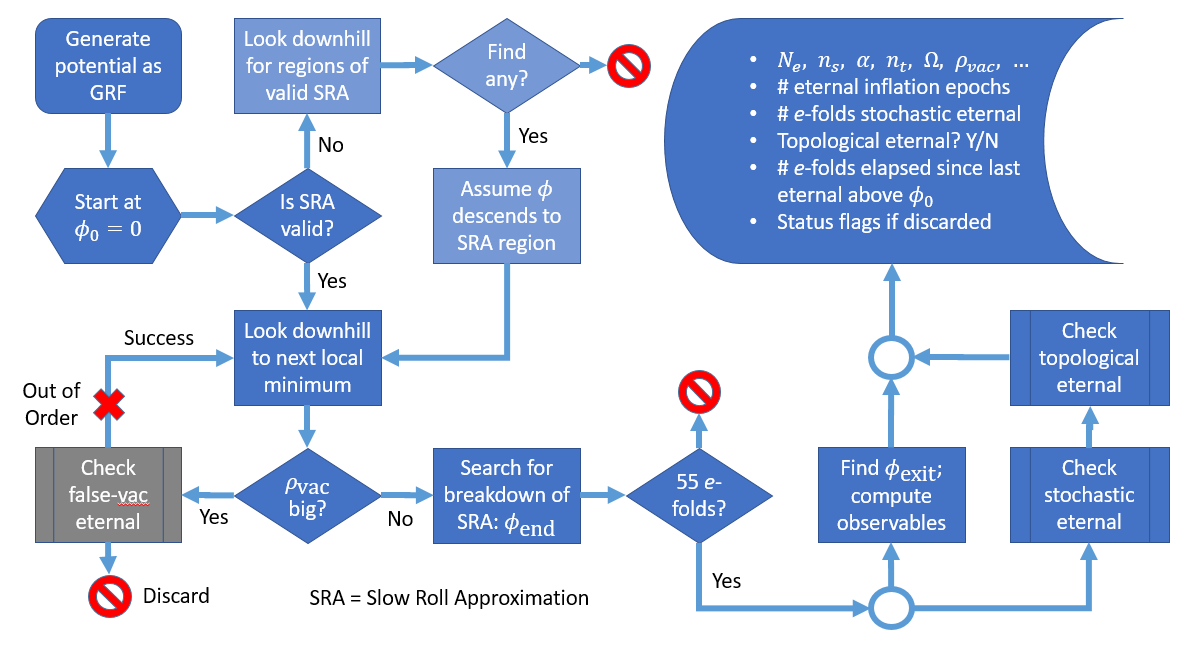
\includegraphics[width=\linewidth]{flowchart}
\end{figure*}

We have reached the limits of applicability of analytical techniques, and now must turn to numerical simulations.

\subsection{Simulating Possible Measures}

% The statement that eternal inflation is or is not generic among a large class of inflation models hides an ambiguity in the choice of measure -– the procedure we adopt for breaking up the space of models for the purpose of assigning probabilities.  The measure establishes the statistical framework in which we assess the likelihood of scenarios like eternal inflation, yet known laws do not appear to single out a preferred measure.  It seems we must make a choice, weighing the merits of possible measures based on factors such as simplicity, alignment with a consistent set of physical principles, and utility in sorting the features that cosmologists are most interested in studying.  

% A measure is a mathematical procedure for assigning a non-negative volume to regions in a space, in such a way that the volume of a subregion is always less than that of its container.  
In the context of inflationary cosmology, we are concerned with measures on the space of viable inflation scenarios -- consisting of a potential function for a single inflaton field and a set of initial conditions (e.g. initial field value).

To explore the consequences of adopting various measures on the space of initial field values, we simulate the dynamics of inflation across an ensemble of randomly generated inflaton potentials.  Following the example of Tegmark, we generate the potential functions as Gaussian random fields.

Since there is always a local maximum to the left and right of any point of the Gaussian random field, there will always be stochastic eternal inflation higher up on the potential slope.

In these simulations, we test for the appearance of stochastic and topological eternal inflation.  Beacuse the Gaussian Random Field has a period much larger than the Planck scale, we could always claim that the field was stuck in a distant false vacuum of the potential before tunneling to the initial value of our simulation.  Searching for false-vacuum eternal inflation would also add enormous costs to the computational complexity of the simulation, since we would need to compute innumerable tunneling amplitudes via an instanton calculation.  We are limiting the simulation to the local half-basin and the half-basins on either side (together a sesqui-basin).  We ignore cases in which inflation ends before the local minimum is reached and the field is able to climb the next hill.

A Gaussian random field (GRF) can be constructed as a superposition of a large number of plane waves, each with the same amplitude and a uniformly distributed random phase.  Following the central limit theorem, the distribution of the field value at any point will approach Gaussian as the number of such plane wave contributions becomes large.  If the potential governing the inflaton owes its form to an interaction with another quantum field.  The Gaussian random potential is (1) bounded from above and below, with arbitrarily large peaks occuring arbitrarily infrequently; (2) contiuous and smooth; and (3) .

We express the potential $V(\phi) = m_v^4 f(\phi/m_h)$ in terms of a dimensionless Gaussian random field
\[ f(x) = \frac{a_0}{2} + \sum_k a_k \cos(kx) + \sum_k a_{-k} \sin(kx) \]
and constants defining the mass scales of the potential ($m_v$) and the field ($m_h$).
The coefficients $a_k$ are sampled from a Gaussian distribution such that 
\[ \text{Var} (a_k) = q^\gamma e^{-q^2/2}, \qquad q \equiv {k}/{k_{\text{max}}} \]

\paragraph{Measure A} The simulation sets the initial field value at $\phi = 0$.

\paragraph{Measure B} Start at the nearest local maximum with $\dot\phi = 0$.

We must enforce constraints so that the observed features of the cosmic microwave background are reproduced by these models.

\begin{enumerate}

\item
Initialize the field according to one of the measures listed above.

\item
Check for topological eternal inflation.  If quantum fluctuations with width $\delta\phi = H/2\pi$ could take the field from its initial value to the nearest local maximum of the potential with probability greater than $ 1/e^3$, evaluate the criterion for topological eternal inflation at that maximum.

\item
Check for stochastic eternal inflation at the maximum.  If the slow roll conditions break down within a Hubble time of classical evolution, then consider approximations invalid -- no stochastic eternal inflation at the maximum.

\item
If the criteria for slow roll inflation are met at the starting point, search the future of the field's classical downhill trajectory for a breakdown of the slow roll conditions.

\item
Evaluate the stochastic eternal inflation criterion \eqref{seic} for field values between the nearest local maximum (past) and the end of slow roll inflation (future).  Record the number of e-foldings that elapse between the breakdown of the SEIC and the end of inflation.

\item
If the field gets trapped in a local minimum, assume that the quantum tunneling rate is sufficiently high, and evaluate the likelihood of false-vacuum eternal inflation.

\end{enumerate}

\begin{figure}
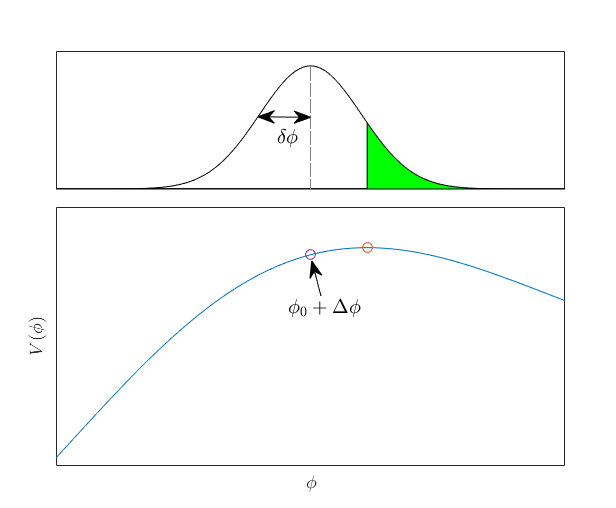
\includegraphics[width=8cm]{topologicalPlot}
\caption{Topological criterion}
\end{figure}
% \[ \sigma_{V^{(k)}(\phi)}^2 = \left( \prod_{i=1}^k \frac{2k-1}{m_h} \right) \sigma_{V(\phi)}^2 \]

\begin{figure}
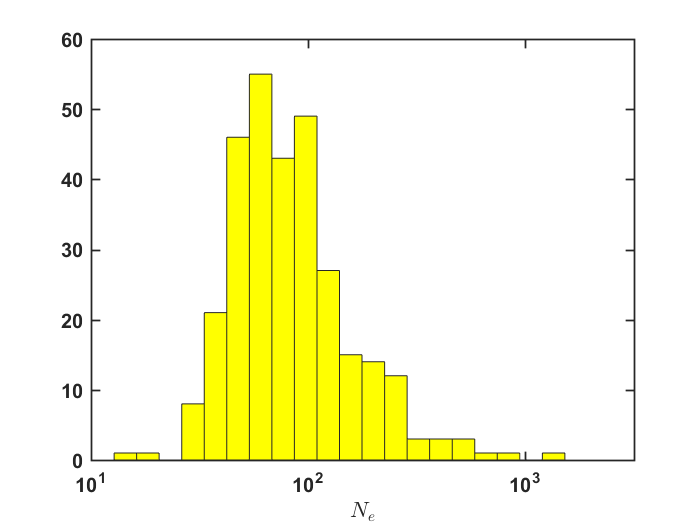
\includegraphics[width=8cm]{NsinceEternal}
\caption{Number of e-foldings elapsed between the breakdown of the stochastic eternal inflation criterion and the starting point. ($m_v = 0.007,\; m_h = 5$)  No constraints were imposed on other parameters.}
\end{figure}

Effects of shifting the potential by $-\rho_\Lambda$:
\begin{align*}
\delta N &= -\int \frac{\rho_\Lambda}{V'} \,\dx \phi \\
\delta Q &= + \mathcal O(\delta \rho_\Lambda^2) \\
\delta r &= 2 r \frac{\rho_\Lambda}{\rho_{\text{exit}}} + \mathcal O(\delta \rho_\Lambda^2) \\
\delta n_s &= \left((n_s - 1) - 6 \epsilon \right) \frac{\rho_\Lambda}{\rho_{\text{exit}}} + \mathcal O(\rho_\Lambda^2) \\
\delta \alpha &= + \mathcal O(\delta \rho_\Lambda^2) \\
\delta n_t &= 2 n_t \frac{\rho_\Lambda}{\rho_{\text{exit}}} + \mathcal O(\delta \rho_\Lambda^2) \\
\delta(\ln \Omega_k) &= + \mathcal O(\delta \rho_\Lambda^2) \\
\delta(\ln \rho) &= + \mathcal O(\delta \rho_\Lambda^2) 
\end{align*}

% \subsection{Genetic Algorithm}

% \begin{enumerate}

% \item
% Randomly generate a population of half-basins of the inflaton potential $V(\phi)$.  These can be generated by first generating a Gaussian random field, and then breaking it up into half-basins.

% \item
% Compute the value of a fitness function for each half-basin, which rewards or penalizes particular characteristics of the potential segment.  For example, the fitness function could maximize the number of e-foldings of inflation.

% \item
% Sort members of the population by fitness.  Breed high performers with other high performers, and discard the worst performers.

% \item
% Check criteria for success at each generation.  Run many iterations of the genetic algorithm, and record the convergence time in each case.  Compare convergence times among different fitness functions to get a relative measure of the genericness of different outcomes.

% \end{enumerate}

We collected the following parameters from each run of the simulation:
\begin{itemize}
\item Number of eternal inflation epochs
\item Duration of each epoch (in e-foldings)
\item If eternal inflation occurred higher up on the potential than the starting point, how many e-foldings of inflation elapsed between the end of the most recent epoch and the starting point.
\item 
\end{itemize}
\paragraph{Next Steps}

\begin{itemize}
\item Enforce constraints on parameters (e.g. $Q_s$, $n_s$) when generating potentials.
\item Express observables ($n_s$, $\alpha_s$, $Q_s$, etc.) in terms of the potential and its derivatives ($V(\phi)$, $V'(\phi)$, etc.).  Compute probability distributions for the potential and its derivatives, and in turn for observables.
\[ n_s = 1 - 6\epsilon + 2\eta = 1 - 3 \left( \frac{V'}{V} \right)^2 + 2 \frac{V''}{V} \]
\[ \alpha = 16\epsilon\eta - 24 \epsilon^2 - 2 \xi_2 \]
\end{itemize}

% \subsection{Designer Inflation Models}

% \paragraph{Genetic Algorithm}

% \paragraph{Optimization}